\chapter{Stars as Quantum Light Sources}
\label{chap:e17}

\begin{chapteropening}
In the previous chapter we translated the various astrophysical radiation mechanisms into quantum language: blackbody, thermal light, and stimulated emission each correspond to particular photon statistics. Now let us point this language at the most ordinary, and most reliable, class of source in the night sky: stars. Their photospheres approximate a surface glowing with thermal light, their angular diameters fall in the milliarcsecond (mas) range, and bright stars deliver enough photons per second to make correlation measurements feasible. Better still, intensity interferometry measures only the correlation of the intensity fluctuations of two telescopes, reading out \(|V|^2\) directly, and requires no optical phase to be maintained between them. This chapter answers one question: when we treat a star no longer as a point but as a glowing surface with structure, what distinct, resolvable fingerprint does each of limb darkening, rapid rotation, circumstellar disks, binarity, and pulsation carve into the \(|V(B)|^2\) curve? Along the way we will recycle the van Cittert--Zernike theorem and the uniform disk of Chapter~\ref{chap:e10}, together with the angular diameter and multi-baseline imaging of Chapter~\ref{chap:e11}, and bring them to bear on VERITAS observations of real stars such as \(\beta\) UMa and \(\gamma\) Cas \citep{1956Natur.177...27B,1974MNRAS.167..121H,1974iiia.book.....H,2020NatAs...4.1164A,2024MNRAS.529.4387A}.
\end{chapteropening}

\section{Why Stars Are the Most Stable Calibration Field}
\label{sec:e17-why-stars}

Start with an intuition: to check whether a ruler is accurate, you measure something whose size you roughly know and that will not move around. Stars are just such an ideal calibrator for the new ruler of quantum astronomy. Under local thermodynamic equilibrium (LTE), the photosphere emits a near-blackbody continuum whose spectral shape and total flux can be described by mature stellar-atmosphere models; bright stars are bright enough that the photon-statistics error can be beaten down by integration time; and their angular diameters fall precisely in the window resolvable by hundred-meter baselines in the visible. Chapter~\ref{chap:e16} already explained that such thermal light satisfies \(g^{(2)}(0)=2\) in a single coherent mode: photons arrive in clumps, with fluctuations twice those of a coherent state.

But the \(g^{(2)}(0)-1\) seen by a real telescope is far smaller than 1. The reason is mode dilution: a single measurement mixes in a large number of spatial, polarization, frequency, and temporal modes, each contributing an independent thermal fluctuation, and the contrast is lowered by the averaging. The quantitative statement given in Chapter~\ref{chap:e08} is the dilution factor \(\zeta\) in the Siegert relation, roughly equal to ``the spacetime volume occupied by a single coherent mode divided by the spacetime volume actually received by the detector.'' On a star, this is not an abstract proposition: a photon-counting intensity interferometry experiment on Vega measured \(\langle g^{(2)}\rangle=1.0034\pm0.0008\) at zero baseline, higher than 1 by only three parts per thousand; on a baseline of about \(2~{\rm km}\) no significant correlation could be measured, fully consistent with Vega's angular diameter of about \(3.3~{\rm mas}\): the star is too large, a kilometer baseline has long resolved it out, and the visibility drops to near zero \citep{2021MNRAS.506.1585Z}. This is what the mode dilution of Chapter~\ref{chap:e08} looks like on a real star.

\paragraph{Intensity correlation directly gives the squared visibility.}
\label{sec:e17-g2-vis}

Intensity interferometry measures the zero-delay correlation of the intensity fluctuations of two telescopes. For thermal light, after subtracting background and applying time-shift normalization, the excess of this correlation is proportional to the squared modulus of one Fourier mode of the sky brightness distribution:
\begin{equation}
  g^{(2)}_{ij}(0)-1 \;=\; |\gamma_{ij}|^2 \;\simeq\; \bigl|V(u_{ij},v_{ij})\bigr|^2 .
  \label{eq:e17-g2-vis}
\end{equation}
\begin{formulaexplain}
\(g^{(2)}_{ij}(0)\): the zero-delay intensity correlation of telescopes \(i,j\). \(\gamma_{ij}\): the complex degree of coherence between the two telescopes. \(V\): the normalized complex visibility, with \((u,v)\) the projected baseline divided by wavelength. This equation says: the excess intensity correlation of thermal light is the squared modulus of a Fourier mode of the sky brightness.
\end{formulaexplain}
Let us account for the symbols one by one. \(g^{(2)}_{ij}(0)\) is dimensionless, the result of multiplying the two photocurrents (or photon counts) at the same instant and normalizing by their respective means; Chapter~\ref{chap:e08} already derived that it is 2 for thermal light and 1 for a coherent state. \(\gamma_{ij}\) is the complex degree of coherence, with modulus between 0 and 1; \((u,v)=\bm{B}_\perp/\lambda\) is the spatial frequency obtained by dividing the projected baseline \(\bm{B}_\perp\) (in cm) by the wavelength \(\lambda\) (in cm), with units of ``wavelengths per radian,'' that is, the number of fringes per radian. The left side of~\eqref{eq:e17-g2-vis} comes from real data processing: delay histogram, time-shift background subtraction, normalized correlation; the right side is the purely geometric Fourier transform of the sky brightness. The crux is that the right side is taken as a squared modulus, so the complex phase is entirely lost. This means \(|V|^2\) is insensitive to overall translation and mirror flip of the sky image (translation only changes the Fourier phase, a mirror takes the complex conjugate, and the squared modulus sees neither). But as long as the target structure itself has a definite geometry (the diameter of a disk, the axis ratio of an ellipse, the separation of a binary pair), these quantities can still be read precisely from \(|V|^2\). This is exactly what every subsequent section of this chapter sets out to do.

\paragraph{Baseline length and angular scale are the same ruler.}
\label{sec:e17-baseline}

To resolve a structure of angular scale \(\theta\), how long a baseline is needed? The answer comes from the most elementary dimensional relation in the van Cittert--Zernike theorem:
\begin{equation}
  B \;\sim\; \frac{\lambda}{\theta}
  \;\simeq\; 103~{\rm m}
  \left(\frac{\lambda}{500~{\rm nm}}\right)
  \left(\frac{\theta}{1~{\rm mas}}\right)^{-1}.
  \label{eq:e17-baseline}
\end{equation}
\begin{formulaexplain}
\(B\): the required baseline length. \(\lambda\): the observing wavelength. \(\theta\): the target angular scale. In the visible, a milliarcsecond star corresponds to a hundred-meter baseline, and kilometer baselines are needed to reach sub-milliarcsecond surface detail.
\end{formulaexplain}
Only by working out this order of magnitude for yourself do you truly understand it. Take \(\lambda=500~{\rm nm}=5\times10^{-7}~{\rm m}\) and \(\theta=1~{\rm mas}\). Converting 1 mas to radians requires multiplying by \(4.848\times10^{-9}\) (because \(1~{\rm arcsec}=1/206265~{\rm rad}\), then dividing by 1000), i.e., \(\theta=4.848\times10^{-9}~{\rm rad}\). Hence
\[
  B\sim\frac{\lambda}{\theta}=\frac{5\times10^{-7}~{\rm m}}{4.848\times10^{-9}}
  \approx 103~{\rm m}.
\]
This is the origin of the coefficient 103 m in~\eqref{eq:e17-baseline}. It tells us that a \(1~{\rm mas}\) star begins to be clearly resolved only with a hundred-meter baseline in the visible; while \(0.1~{\rm mas}\) surface structure (such as rotational oblateness or starspots) requires kilometer-scale baselines. Historically the Narrabri intensity interferometer used variable baselines of \(10\)--\(188~{\rm m}\) and two \(6.7~{\rm m}\) reflectors to measure the angular diameters of 32 bright stars \citep{1974MNRAS.167..121H,1974iiia.book.....H}. Today VERITAS, MAGIC, and the future CTA-class arrays, with Cherenkov telescopes of \(>10~{\rm m}\) aperture, larger light-collecting area, and digital correlators, have reopened this parameter space \citep{2020NatAs...4.1164A,2024MNRAS.529.4387A}.

The scaling of the signal-to-noise ratio was given in full in Eq.~\eqref{eq:e11-snr} of Chapter~\ref{chap:e11}; here we only name its direct implication for stellar target selection: the higher the photon rate, the larger the electronic bandwidth, and the longer the integration, the smaller the error on \(|V|^2\) (the signal-to-noise ratio grows only as the square root of integration time); while background light, detector dead time, finite time resolution, and systematic covariance determine where this statistical gain ceases to ``pay off.'' So the first targets naturally lean toward bright, hot, blue stars whose angular diameters are already resolvable at hundred-meter baselines \citep{2013MNRAS.430.3187R,2020NatAs...4.1164A}. This is not a slogan; it is the physical basis for the ``how to lay out baselines'' of the next section.

\section{Reading Angular Diameter and Temperature from the Squared Visibility}
\label{sec:e17-diameter-teff}

The first step from data to radius is to treat the star, provisionally, as a ``uniformly glowing coin,'' with a single parameter: the angular diameter \(\theta\). This is the uniform disk model of Chapter~\ref{chap:e10}, whose visibility is given by Eq.~\eqref{eq:e10-disk},
\[
  V_{\rm UD}(B)=\frac{2J_1(x)}{x},\qquad x=\frac{\pi\theta B}{\lambda},
\]
where \(J_1\) is the first-order Bessel function and \(x\) is the dimensionless ``degree of resolution.'' Here \(B\) is the projected baseline, \(\lambda\) is the effective wavelength, and \(\theta\) must be in radians (if given in mas, multiply by \(4.848\times10^{-9}\)). Intensity interferometry fits \(|V_{\rm UD}|^2\), the complex phase already erased by the squared modulus. The most information-dense place on the curve is near the first null (\(x=3.8317\), corresponding to \(B_0\approx1.22\lambda/\theta\)): there \(|V|^2\) is most sensitive to the angular diameter; but near the null \(|V|^2\) is so small that background and systematic errors can swamp the signal. So a real measurement must cover short, intermediate, and long baseline segments: short baselines fix the total flux and the correlation normalization, intermediate baselines give the falling slope that yields the diameter, and long baselines test whether the model still needs limb darkening, oblateness, or a companion.

\begin{figure}[tbp]
\centering
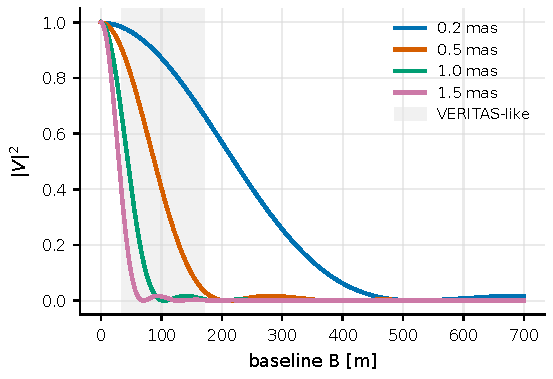
\includegraphics[width=0.82\linewidth]{figures/generated/chapter_10/ch10_stellar_diameter_visibility.pdf}
\caption{The \(|V|^2\) of a uniform-disk star versus baseline. The wavelength is taken as \(416~{\rm nm}\), close to the observing wavelength of VERITAS intensity interferometry. The larger the angular diameter, the faster the visibility falls; the gray region marks the VERITAS-scale projected-baseline range of \(35\)--\(170~{\rm m}\), suited to measuring bright stars of about \(0.5\)--\(1.5~{\rm mas}\).}
\label{fig:e17-diameter-visibility}
\end{figure}

\paragraph{Angular diameter plus total flux equals effective temperature.}
\label{sec:e17-teff}

Once the angular diameter is measured, knowing this star's total radiant flux at Earth is all it takes to obtain its effective temperature. The derivation needs only the Stefan--Boltzmann law plus one step of geometry. The stellar luminosity is \(L=4\pi R^2\sigma_{\rm SB}T_{\rm eff}^4\), where \(R\) is the radius. Propagated to distance \(d\), the bolometric flux received at Earth is \(F_{\rm bol}=L/(4\pi d^2)=R^2\sigma_{\rm SB}T_{\rm eff}^4/d^2\). And the relation between angular diameter and radius is \(\theta_{\rm LD}=2R/d\), i.e., \(R/d=\theta_{\rm LD}/2\), so \(R^2/d^2=\theta_{\rm LD}^2/4\). Substituting back, the distance \(d\) cancels automatically:
\begin{equation}
  F_{\rm bol}=\frac{\theta_{\rm LD}^2}{4}\,\sigma_{\rm SB}T_{\rm eff}^4,
  \qquad
  T_{\rm eff}=\left(\frac{4F_{\rm bol}}{\sigma_{\rm SB}\theta_{\rm LD}^2}\right)^{1/4}.
  \label{eq:e17-teff}
\end{equation}
\begin{formulaexplain}
\(F_{\rm bol}\): the total radiant flux measured at Earth (\({\rm erg\,s^{-1}\,cm^{-2}}\)). \(\theta_{\rm LD}\): the limb-darkened angular diameter. \(\sigma_{\rm SB}\): the Stefan--Boltzmann constant. Angular diameter and total flux together fix the effective temperature without any need to know the distance.
\end{formulaexplain}
Note the beautiful feature: the distance \(d\) is cancelled out in the derivation, so \(T_{\rm eff}\) is a quantity ``independent of the distance scale'': you need only measure the angular diameter and the flux. The subscript LD on \(\theta_{\rm LD}\) reminds us that the limb-darkened angular diameter should be used here (the next section explains why the uniform-disk diameter cannot), in radians or mas; \(\sigma_{\rm SB}=5.67\times10^{-5}~{\rm erg\,s^{-1}\,cm^{-2}\,K^{-4}}\) (CGS).

For the same star, we care more about how the measurement error propagates to \(T_{\rm eff}\). Since \(T_{\rm eff}\propto F_{\rm bol}^{1/4}\theta_{\rm LD}^{-1/2}\), taking logarithms gives \(\ln T_{\rm eff}=\tfrac14\ln F_{\rm bol}-\tfrac12\ln\theta_{\rm LD}+{\rm const}\). Differentiating: \({\rm d}\ln T_{\rm eff}=\tfrac14\,{\rm d}\ln F_{\rm bol}-\tfrac12\,{\rm d}\ln\theta_{\rm LD}\). If the errors of \(F_{\rm bol}\) and \(\theta_{\rm LD}\) are independent, the variances add in quadrature and the coefficients are squared:
\begin{equation}
  \left(\frac{\sigma_T}{T_{\rm eff}}\right)^2
  \simeq
  \frac{1}{16}\left(\frac{\sigma_F}{F_{\rm bol}}\right)^2
  +\frac{1}{4}\left(\frac{\sigma_\theta}{\theta_{\rm LD}}\right)^2 .
  \label{eq:e17-teff-error}
\end{equation}
\begin{formulaexplain}
\(\sigma_T,\sigma_F,\sigma_\theta\): the absolute errors of temperature, total flux, and angular diameter. Because \(T_{\rm eff}\propto F_{\rm bol}^{1/4}\theta_{\rm LD}^{-1/2}\), for the same percentage error the angular-diameter term (coefficient \(1/4\)) carries four times the weight of the flux term (coefficient \(1/16\)).
\end{formulaexplain}
The coefficients \(1/16=(1/4)^2\) and \(1/4=(1/2)^2\) are precisely the squares of the exponents. The conclusion: the relative error of the angular diameter enters \(T_{\rm eff}\) with four times the weight of the flux, so the angular diameter often dominates the temperature precision. This is exactly the value of intensity interferometry: it turns an angular diameter that was once inferred indirectly through models into a direct measurement. VERITAS intensity-interferometry observations of \(\beta\) Ursae Majoris (\(\beta\) UMa) gave \(\theta_{\rm LD}=1.07\pm0.04\,({\rm stat})\pm0.05\,({\rm sys})~{\rm mas}\), which substituted into~\eqref{eq:e17-teff} yields \(T_{\rm eff}\simeq9700\pm200\pm200~{\rm K}\), and can further constrain the age of the Ursa Major moving group \citep{2024ApJ...966...28A}. And the two bright blue stars \(\beta\) Canis Majoris (\(\beta\) CMa) and \(\epsilon\) Orionis (\(\epsilon\) Ori), measured in the first modern VERITAS intensity-interferometry survey, are exactly the opening act of this method in the real sky \citep{2020NatAs...4.1164A}.

\begin{figure}[tbp]
\centering
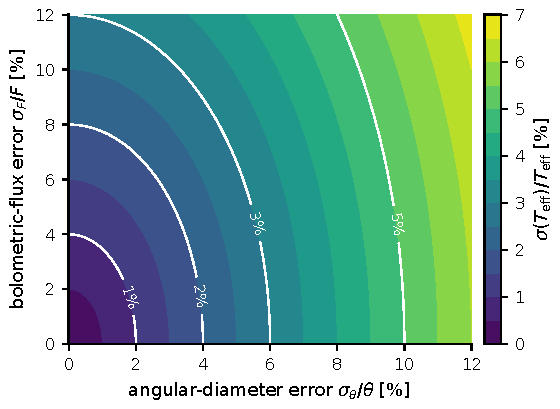
\includegraphics[width=0.78\linewidth]{figures/generated/chapter_10/ch10_teff_error_budget.pdf}
\caption{Error propagation for deriving \(T_{\rm eff}\) from \(F_{\rm bol}\) and \(\theta_{\rm LD}\). The horizontal axis is the relative error of the angular diameter, the vertical axis the relative error of the total flux, and color gives the relative error of the effective temperature. Because \(T_{\rm eff}\propto F_{\rm bol}^{1/4}\theta_{\rm LD}^{-1/2}\), an angular-diameter error is usually more ``valuable'' than a flux error of the same percentage.}
\label{fig:e17-teff-error}
\end{figure}

\paragraph{Add the distance to get radius and luminosity.}
\label{sec:e17-radius}

If this star's distance \(d\) is given independently by the Gaia parallax, then the angular diameter can be translated into a physical radius, and the Stefan--Boltzmann law then gives the luminosity:
\begin{equation}
  R=\frac{1}{2}\theta_{\rm LD}\,d,\qquad
  L=4\pi R^2\sigma_{\rm SB}T_{\rm eff}^4 .
  \label{eq:e17-radius}
\end{equation}
\begin{formulaexplain}
\(R\): the physical stellar radius. \(d\): the distance. \(L\): the luminosity. The angular diameter gives ``how large on the sky,'' the distance turns it into ``how large in reality,'' and the Stefan--Boltzmann law then gives ``how bright it shines.''
\end{formulaexplain}
The first equation is just a rewriting of \(\theta_{\rm LD}=2R/d\); \(\theta_{\rm LD}\) is in radians, and \(d\) and \(R\) are in the same unit (both cm, say, or if \(d\) is in pc and \(R\) in \(R_\odot\), remember to convert). Combining the Gaia parallax, the intensity-interferometry angular diameter, and \(F_{\rm bol}\), a star falls into a small region with covariance on the Hertzsprung--Russell (HR) diagram. Comparing this small region with stellar evolutionary tracks constrains the mass, age, and model parameters such as the mixing length, convective overshoot, and rotation. The infrared flux method, the angular diameters from amplitude interferometers such as Mark III and CHARA, and the intensity-interferometry angular diameters are, at this level, mutually corroborating independent rulers \citep{1977MNRAS.180..177B,1991AJ....101.2207M,1994A&A...282..899B,2003AJ....126.2502M,2005ApJ...626..446R}.

\section{Why Limb Darkening Is Not a Small Correction}
\label{sec:e17-limb-darkening}

Treating the star as a uniform coin incurs a debt that must be repaid: the edge of a real stellar disk is darker. The reason is very physical: when you look toward the disk center, the line of sight plunges vertically into the atmosphere and sees the deeper, hotter layers; when you look toward the edge, the line of sight grazes at a steep angle and sees only the shallower, cooler upper layers. Lower temperature means lower brightness, so the edge grows dark; this is limb darkening. The simplest linear model is
\begin{equation}
  I(\mu)=I(1)\,[1-u_\lambda(1-\mu)],
  \qquad
  \mu=\sqrt{1-r^2}.
  \label{eq:e17-linear-ld}
\end{equation}
\begin{formulaexplain}
\(I(\mu)\): the surface brightness at different viewing angles. \(\mu\): the cosine of the angle between the surface normal and the line of sight. \(r\): the normalized projected radius (center \(r=0\), edge \(r=1\)). \(u_\lambda\): the wavelength-dependent limb-darkening coefficient. It compresses ``the edge darkens'' into a single parameter.
\end{formulaexplain}
Term by term: \(r\) is the radius on the projected disk divided by the stellar radius, ranging from 0 to 1; at the center the line of sight is perpendicular and \(\mu=1\), at the edge it grazes and \(\mu=0\), the geometric relation being precisely \(\mu=\sqrt{1-r^2}\). \(I(1)\) is the central brightness. \(u_\lambda\) is the limb-darkening coefficient: \(u_\lambda=0\) reverts to the uniform disk, and the larger \(u_\lambda\), the darker the edge; it is dimensionless and depends strongly on wavelength: for a hot star in the blue, a cool giant in a molecular absorption band, or a Mira variable at different pulsation phases, \(u_\lambda\) all differ. Modern analyses usually do not use this linear form but instead generate a synthetic \(I(\mu)\) directly from an atmosphere model and then compute the visibility; the linear \(u_\lambda\) is used mainly for order-of-magnitude estimates and intuition \citep{1974MNRAS.167..475H,1992A&A...259..227D,1997A&A...327..199H,2015MNRAS.453.3821P}.

\paragraph{The visibility of any radial profile is a Hankel transform.}
\label{sec:e17-hankel}

To learn how limb darkening changes the visibility curve, we need a formula that can accept ``any radial brightness profile.'' For any axisymmetric (circularly symmetric) brightness distribution \(I(r)\), its visibility is the radial Hankel transform:
\begin{equation}
  V(x)=
  \frac{\displaystyle\int_0^1 I(r)\,J_0(xr)\,r\,{\rm d}r}
       {\displaystyle\int_0^1 I(r)\,r\,{\rm d}r},
  \label{eq:e17-hankel}
\end{equation}
\begin{formulaexplain}
\(V(x)\): the visibility of an axisymmetric brightness distribution. \(J_0\): the zeroth-order Bessel function. \(x\): the dimensionless spatial frequency assembled from baseline, wavelength, and angular radius. The denominator is the normalization (total flux), and the numerator projects the brightness profile onto that frequency.
\end{formulaexplain}
Where does this equation come from? When a two-dimensional Fourier transform acts on a circularly symmetric function, the azimuthal integral \(\int_0^{2\pi}e^{-i x r\cos\phi}\,{\rm d}\phi=2\pi J_0(xr)\): this is the integral representation of the zeroth-order Bessel function, a standard result, which reduces the two-dimensional Fourier transform directly to a one-dimensional radial integral. The denominator \(\int_0^1 I(r)\,r\,{\rm d}r\) is the total flux, ensuring \(V(0)=1\). The uniform disk is the special case \(I(r)={\rm const}\): here the numerator uses another standard result \(\int_0^1 J_0(xr)\,r\,{\rm d}r=J_1(x)/x\), the denominator is \(1/2\), and dividing one by the other returns exactly to \(V=2J_1(x)/x\), i.e., Eq.~\eqref{eq:e10-disk}. Substituting the linear profile with \(u_\lambda>0\), the darkened edge makes the disk boundary no longer ``sharp,'' with the effect of pushing the first null of the visibility outward and lowering the height of the first sidelobe.

\begin{figure}[tbp]
\centering
\includegraphics[width=0.92\linewidth]{figures/generated/chapter_10/ch10_limb_darkening.pdf}
\caption{The effect of linear limb darkening on surface brightness and visibility. The left panel shows the radial brightness profile for the three cases \(u_\lambda=0,0.4,0.8\); the right panel shows the corresponding \(|V|^2\) obtained by numerically integrating Eq.~\eqref{eq:e17-hankel}. The darker the edge, the more blurred the disk boundary, and the positions of the visibility nulls and sidelobes shift accordingly.}
\label{fig:e17-limb-darkening}
\end{figure}

This is precisely why limb darkening is not a ``drawing detail'' but a source of systematic error: for the same set of \(|V|^2\) data, fitting with a uniform disk gives \(\theta_{\rm UD}\), while fitting with a limb-darkened atmosphere model gives \(\theta_{\rm LD}\), closer to the true photospheric boundary, and the two can differ by a few percent. What it changes is not whether the curve looks nice but ``which radius you are actually measuring.'' Back then, the Narrabri angular-diameter catalog had to correct the uniform-disk diameter into a limb-darkened diameter before temperature and radius could be discussed further \citep{1974MNRAS.167..121H,1974MNRAS.167..475H}. For intensity interferometry, the calibration error must further stack together the effects of the catalog angular diameter, correlator gain, time synchronization, background light, and \(|V|^2\) covariance; each item must be accounted for separately.

\section{How Rotation, Binarity, and Surface Structure Enter the Visibility}
\label{sec:e17-rotation-binary}

So far the star has still been a circle. In reality it may be flattened by rotation, may have a companion, may be mottled on its surface. These structures write non-circular, non-symmetric information into \(|V|^2\), and we examine what each fingerprint looks like in turn.

\paragraph{Rapid rotation: oblateness and gravity darkening.}
\label{sec:e17-rotation}

A rapidly rotating star has its equator flung outward by centrifugal force, and the photosphere goes from a sphere to an oblate spheroid. More subtly, there is gravity darkening: with the equator bulged out, the surface gravity there decreases, and so does the surface temperature there, so the equator is darker and cooler than the poles. The first geometric effect is that the projection is an ellipse. Approximating the projected photosphere as an ellipse, the effective angular diameter seen along the baseline direction \(\psi\) is
\begin{equation}
  \theta_{\rm eff}^2(\psi)=
  \theta_{\rm maj}^2\cos^2\psi+
  \theta_{\rm min}^2\sin^2\psi ,
  \label{eq:e17-ellipse}
\end{equation}
\begin{formulaexplain}
\(\theta_{\rm eff}(\psi)\): the effective angular diameter seen along the baseline direction \(\psi\). \(\theta_{\rm maj},\theta_{\rm min}\): the major- and minor-axis angular diameters of the projected ellipse. Rotational oblateness makes the falling rate of \(|V|^2\) vary with position angle.
\end{formulaexplain}
This equation is just the ``apparent width'' formula for an ellipse in direction \(\psi\): when the baseline is along the major axis (\(\psi=0\)) then \(\theta_{\rm eff}=\theta_{\rm maj}\), the star looks ``widest'' and the visibility falls fastest; along the minor axis (\(\psi=90^\circ\)) then \(\theta_{\rm eff}=\theta_{\rm min}\), and the visibility falls slowest. So a baseline of the same length, pointed at different position angles, reads different \(|V|^2\): this is the resolvable fingerprint left by oblateness. This is exactly how VERITAS intensity-interferometry observations of \(\gamma\) Cassiopeiae (\(\gamma\) Cas) at \(416~{\rm nm}\) measured the oblateness: minor-axis angular diameter \(0.43\pm0.02~{\rm mas}\), major-to-minor radius ratio \(1.28\pm0.04\), position angle \(116^\circ\pm5^\circ\); then using a rapid-rotation atmosphere model, they further gave a lower bound on the rotation velocity close to breakup and an equatorial radius of about \(10.9~R_\odot\) \citep{2025ApJ...995..191A}.

\begin{figure}[tbp]
\centering
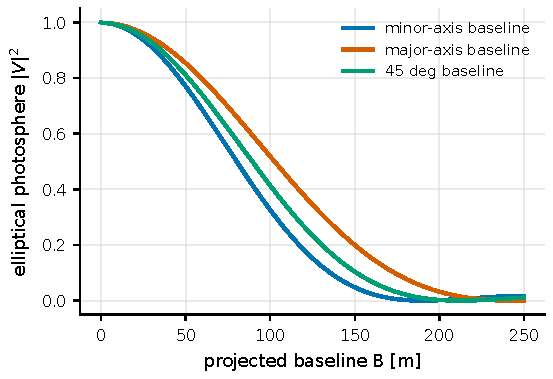
\includegraphics[width=0.82\linewidth]{figures/generated/chapter_10/ch10_rotation_oblateness.pdf}
\caption{The \(|V|^2\) of a rapidly rotating elliptical photosphere along different baseline directions. Parameters are taken at the \(\gamma\) Cas-scale axis ratio of \(1.28\) and \(416~{\rm nm}\) wavelength. Projected along different position angles, the effective angular diameter differs, so the same baseline length gives a different correlation strength; this geometric effect lets intensity interferometry measure the photospheric oblateness directly.}
\label{fig:e17-rotation}
\end{figure}

\paragraph{Binaries: cosine oscillations in visibility space.}
\label{sec:e17-binary}

A pair of close binary stars, neither yet resolved individually, overlays a layer of cosine ripples on the visibility curve. The derivation is direct: treat the two stars as two point sources, the primary flux taken as 1, the secondary as \(f\) (the flux ratio), with angular separation vector \(\bm{d}\). The visibility of two point sources is the weighted sum of their complex phases, \(V=(1+f\,e^{i\phi})/(1+f)\), where the phase \(\phi=2\pi\bm{u}\cdot\bm{d}\) comes from the optical path difference of the two point sources. Taking the squared modulus: \(|1+f e^{i\phi}|^2=(1+f\cos\phi)^2+(f\sin\phi)^2=1+f^2+2f\cos\phi\). Dividing by the normalization \((1+f)^2\):
\begin{equation}
  |V_{\rm bin}|^2=
  \frac{1+f^2+2f\cos(2\pi\bm{u}\cdot\bm{d})}
       {(1+f)^2}.
  \label{eq:e17-binary}
\end{equation}
\begin{formulaexplain}
\(|V_{\rm bin}|^2\): the squared visibility of an unresolved binary. \(f\): the flux ratio of secondary to primary. \(\bm{u}=\bm{B}_\perp/\lambda\): the spatial frequency. \(\bm{d}\): the angular separation vector (radians). The cosine term makes the binary oscillate in baseline space.
\end{formulaexplain}
Reading this equation: the oscillation period is set by \(\bm{u}\cdot\bm{d}\): the larger the separation \(\bm{d}\) and the longer its projection along the baseline, the faster it oscillates with baseline, so the angular separation along the baseline direction can be inferred from the oscillation period; the depth of the oscillation is set by \(f\), and when \(f\to1\) (two equally bright stars) the coefficient of the cosine term \(2f/(1+f)^2\to1/2\) is maximal and the ripples are deepest, while for \(f\to0\) (a very faint secondary) the ripples vanish. If the two stars are each partially resolved, one need only multiply each term by its own disk visibility, Eq.~\eqref{eq:e10-disk}. Some targets in the Narrabri catalog were later recognized as binaries or multiples; modern multi-baseline intensity-interferometry arrays can jointly fit the binary orbit, angular diameters, and brightness ratio, and combined with radial velocities determine the masses \citep{1970MNRAS.148..103H,1974MNRAS.167..121H,2012MNRAS.419..172N}.

\begin{figure}[tbp]
\centering
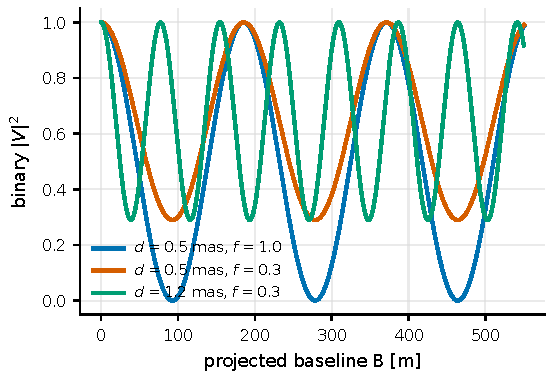
\includegraphics[width=0.82\linewidth]{figures/generated/chapter_10/ch10_binary_visibility.pdf}
\caption{The \(|V|^2\) oscillation of an unresolved binary. The larger the angular separation, the faster the oscillation with baseline; the closer the flux ratio to 1, the larger the oscillation amplitude. A real binary further requires the finite angular diameters of the two stars, the orbital position angle, and the multi-wavelength flux ratio.}
\label{fig:e17-binary}
\end{figure}

\paragraph{Surface structure: the degeneracy brought by missing phase.}
\label{sec:e17-surface}

Surface structure is thornier than binarity, because \(|V|^2\) lacks phase. Starspots, large convective granules, non-radial pulsations, and Be-star disks all introduce non-axisymmetric signals; if one merely fits a disk or binary model, one may well get a result that ``fits the curve beautifully but is physically wrong,'' exactly the model degeneracy caused by missing phase. The way to break it is to add dimensions of constraint: multiple baselines, multiple nights, multiple wavelengths, and spectral-line channels can each suppress part of the degeneracy. Simulation studies show that a Cherenkov telescope array, with enough baseline number and coverage, has a chance to reconstruct diameter, oblateness, binary structure, and even large-scale surface features; but to reconstruct a genuinely complex image still requires prior information or joint use with amplitude-interferometry data \citep{2012MNRAS.419..172N,2013MNRAS.430.3187R}.

\section{How Time Variation and Spectral-Line Channels Extend the Stellar Image}
\label{sec:e17-time-line}

The stars so far have all been ``static.'' The final section lets stars move and lets different wavelengths speak for themselves, to see what more intensity interferometry can measure.

\paragraph{Cepheids: connecting the angular-radius change to the distance scale.}
\label{sec:e17-cepheid}

A Cepheid variable periodically swells and shrinks, and its angular diameter changes with pulsation phase. This gives a ruler for the heavens independent of parallax: the Baade--Wesselink class of methods. The idea is: the radial-velocity spectral lines tell us the surface velocity along the line of sight, and integrating it gives the physical change in radius \(\Delta R\); while intensity interferometry directly measures the change in angular radius \(\Delta\theta\). The ratio of the two is the distance. Quantitatively, first fix conventions: the radial velocity \(v_r\) is positive away from us (redshift positive), and when the surface expands toward us the line is blueshifted, \(v_r-v_\gamma<0\), while the radius is then increasing, so the rate of change of radius and the radial pulsation velocity differ by a minus sign,
\[
  \frac{{\rm d}R}{{\rm d}t}=-p\,[v_r(t)-v_\gamma].
\]
Integrating both sides over time gives the physical change in radius
\[
  \Delta R(t)=-\int p\,[v_r(t)-v_\gamma]\,{\rm d}t.
\]
Using the geometric relation between angular diameter and radius \(\Delta\theta=2\Delta R/d\) and substituting gives
\begin{equation}
  \Delta\theta(t)=-\frac{2}{d}
  \int p\,[v_r(t)-v_\gamma]\,{\rm d}t .
  \label{eq:e17-baade-wesselink}
\end{equation}
\begin{formulaexplain}
\(\Delta\theta(t)\): the change of angular diameter with time. \(d\): the distance. \(v_r-v_\gamma\): the radial pulsation velocity after subtracting the overall systemic velocity (positive away). \(p\): the projection factor converting the observed radial velocity into the true pulsation velocity. The minus sign is a consequence of the velocity sign convention; the actual analysis cares only about the amplitude and phase of \(\Delta\theta(t)\), the sign fixed by convention.
\end{formulaexplain}
Term by term: \(v_r(t)\) is the radial velocity measured from the spectral lines, \(v_\gamma\) is the systemic velocity of the whole star relative to us (a constant), and it is their difference that is the pulsation itself. The minus sign in the equation comes purely from the sign convention ``radial velocity positive away, while expansion brings the surface toward us''; switch conventions and the sign flips, and in a real distance fit only the shape (amplitude and phase) of the \(\Delta\theta(t)\) curve is used, so the sign does not affect the result, but getting it right keeps the main-text derivation and the boxed formula internally consistent. \(p\) is the projection factor, because a spectral line is a radial-velocity-weighted average over the whole visible hemisphere, whereas what we want is the true radial expansion velocity of the surface, the two differing by a geometric factor of order \(1.3\). Once the angular-diameter curve \(\Delta\theta(t)\) is phase-matched to the velocity-integral curve, the only free scale left is \(d\), and the distance is thereby fixed. The systematic errors come from the \(p\)-factor, limb darkening (\(u_\lambda\) changes during pulsation), companion contamination, period changes, and atmospheric velocity gradients. Bright Cepheids are especially tempting for visible-light intensity interferometry: they are both bright and have a predictable radius change \citep{1997A&A...320..799F,2007A&A...476...73F}.

\paragraph{Spectral-line channels: separating the structure of the continuum and line regions.}
\label{sec:e17-line}

For Be stars and Wolf--Rayet stars, the continuum comes from the photosphere while the emission lines come from an extended disk or wind, the two on different spatial scales. If a narrowband filter frames the continuum and an emission line at once, the observed visibility is the flux-weighted sum of the two:
\begin{equation}
  V_{\rm obs}=
  \frac{F_{\rm cont}V_{\rm cont}+F_{\rm line}V_{\rm line}}
       {F_{\rm cont}+F_{\rm line}} .
  \label{eq:e17-line-visibility}
\end{equation}
\begin{formulaexplain}
\(V_{\rm obs}\): the net visibility observed within the narrow band. \(F_{\rm cont},F_{\rm line}\): the fluxes of the continuum and the line. \(V_{\rm cont},V_{\rm line}\): their respective visibilities. If the continuum is already calibrated, one can invert for the visibility of the line-forming region and hence its spatial scale.
\end{formulaexplain}
The physical basis of this equation is that the two components are mutually incoherent: the continuum comes from the photosphere and the emission line from the extended disk or wind, they are photons emitted from different regions by different processes, and they have no fixed phase relation. Mutual incoherence means their intensities add directly, the cross interference term averages to zero over time, and so the mutual coherence function (i.e., the visibility) is linearly weighted by their respective fluxes, giving Eq.~\eqref{eq:e17-line-visibility}; no assumption of coherent field superposition is needed. The use is very practical: first fix \(V_{\rm cont}\) using an adjacent pure-continuum band (that is the photospheric disk), then subtract it from Eq.~\eqref{eq:e17-line-visibility} to invert for the \(V_{\rm line}\) of the line region, thereby constraining the disk radius, inclination, or wind geometry. For rapidly rotating Be stars, the H\(\alpha\) line outlines the disk while the blue continuum outlines the photosphere; \(\gamma\) Cas is a paradigm: intensity interferometry directly measured the photospheric oblateness, while infrared or H\(\alpha\) interferometry supplies the geometry of the disk \citep{2025ApJ...995..191A}.

The last special case is the astrophysical laser and stimulated spectral lines, which may appear in systems like \(\eta\) Carinae where a strong radiation field coexists with dense gas clumps. To prove that a spectral line comes from stimulated emission, line strength alone is not enough; one needs simultaneously the line width, spatial position, pumping channel, polarization, and the \(g^{(2)}\) in the line channel: stimulated emission pushes the photon statistics from the clumping of thermal light (\(g^{(2)}>1\)) toward the Poisson of a coherent state (\(g^{(2)}\to1\)). The quantum diagnostics of the astrophysical laser discussed in Chapter~\ref{chap:e16} land here as a concrete target-selection checklist \citep{2004A&A...428..497J,2005NewA...10..361J,2008AIPC..984..216D}.

\section{Chapter Summary}
\label{sec:e17-summary}

\begin{itemize}
  \item \textbf{Stars are the most stable calibration field.} The photosphere approximates thermal light, bright stars have adequate photon rates, and the angular diameter is in the milliarcsecond range; intensity interferometry reads \(|V|^2\) directly (Eq.~\eqref{eq:e17-g2-vis}), with no need to maintain optical phase between telescopes. Mode dilution makes the measured \(g^{(2)}(0)-1\) very small: Vega at zero baseline gives only \(1.0034\pm0.0008\).
  \item \textbf{Baseline and angular scale are the same ruler.} \(B\sim\lambda/\theta\): in the visible \(1~{\rm mas}\) corresponds to about 103 m, and \(0.1~{\rm mas}\) surface structure requires kilometer-scale baselines (Eq.~\eqref{eq:e17-baseline}).
  \item \textbf{Angular diameter plus flux gives temperature.} \(F_{\rm bol}=(\theta_{\rm LD}^2/4)\sigma_{\rm SB}T_{\rm eff}^4\), with distance cancelled out (Eq.~\eqref{eq:e17-teff}); the relative error of the angular diameter carries four times the weight of the flux in \(T_{\rm eff}\) (Eq.~\eqref{eq:e17-teff-error}). VERITAS gave \(\theta_{\rm LD}=1.07~{\rm mas}\), \(T_{\rm eff}\simeq9700~{\rm K}\) for \(\beta\) UMa.
  \item \textbf{Limb darkening changes ``which radius.''} The visibility of any axisymmetric profile is a Hankel transform (Eq.~\eqref{eq:e17-hankel}); the uniform-disk diameter \(\theta_{\rm UD}\) and the limb-darkened diameter \(\theta_{\rm LD}\) can differ by a few percent, a systematic error rather than a drawing detail.
  \item \textbf{Rotation, binarity, and surface structure each have a fingerprint.} Oblateness makes \(|V|^2\) vary with position angle (Eq.~\eqref{eq:e17-ellipse}, \(\gamma\) Cas axis ratio 1.28); a binary overlays a cosine oscillation (Eq.~\eqref{eq:e17-binary}); surface structure is easily degenerate due to missing phase, broken by multiple baselines, wavelengths, and nights.
  \item \textbf{Time and spectral lines extend the image.} The Cepheid angular-radius change connects to the Baade--Wesselink distance (Eq.~\eqref{eq:e17-baade-wesselink}); within a narrow band the continuum and line are flux-weighted (Eq.~\eqref{eq:e17-line-visibility}), separating photosphere from disk.
\end{itemize}

\noindent\textbf{Questions to Ponder.}
\begin{itemize}
  \item For a \(0.5~{\rm mas}\) bright star at \(416~{\rm nm}\), at roughly what baseline is the first null? (Hint: \(B_0\approx1.22\lambda/\theta\).) If you have only \(35\)--\(170~{\rm m}\) baselines, can you reach the null? What is the effect on the fitted angular diameter of not reaching it?
  \item If the angular separation of two equally bright binary stars (\(f=1\)) is \(1~{\rm mas}\) along some direction, what baseline interval corresponds to the period of the cosine term in Eq.~\eqref{eq:e17-binary}? How does this period change after rotating the position angle by \(90^\circ\)?
  \item Why is \(T_{\rm eff}\) in Eq.~\eqref{eq:e17-teff} independent of distance, while \(R\) and \(L\) in Eq.~\eqref{eq:e17-radius} depend on it? What does this imply for the observing strategy of ``measure temperature first or radius first''?
\end{itemize}
